\documentclass[russian]{article}
\usepackage[T1]{fontenc}
\usepackage[utf8]{inputenc}
\usepackage{geometry}
\geometry{verbose,tmargin=2cm,bmargin=2cm,lmargin=1cm,rmargin=1cm}
\usepackage{float}
\usepackage{textcomp}
\usepackage{amssymb}
\usepackage{graphicx}
\usepackage{babel}
\usepackage[T2A]{fontenc}

\makeatletter
\@ifundefined{date}{}{\date{}}


\begin{document}

\title{Теория графов. HW\#6}
\author{Тураев Тимур, 504 (SE)}

\maketitle

\paragraph{0.} \textit{Во всех последующих задачах будет активно использоваться задача 6.18 (про существование $k$-веера в $k$-связном графе). Меня на прошлом занятии не было, но, говорят, что эта задача была решена.}

Если это не так, то решается-то она довольно просто. 

Берем такой $k$-связный граф, выбираем согласно условию вершину $x$, множество $Y$, состоящее из не менее чем $k$ вершин графа, не содержащее $x$. Далее, добавляем в граф новую вершину $y$ и соединяем ребрами ее с какими-нибудь $k$ вершинами из множества $Y$.

Согласно задаче 6.17 (которая точно была решена), граф остается $k$-связным. По теореме Менгера в этом графе между вершинами $x$ и $y$ существует $k$ непересекающихся путей (здесь и далее под <<непересекающимися>> путями будем понимать пути, не имеющие общих внутренних точек). Очевидно, что эти пути будут проходить через те выбранные $k$ вершин во множестве $Y$ и заканчиваться <<новыми>> ребрами, ведущими в вершину $y$.

Затем удалим вершину $y$ из графа и получим то что требуется: $k$-веер из $x$ в $Y$.

\paragraph{1.} \textit{С помощью теоремы Менгера докажите, что $k$-мерный гиперкуб $k$-связен.}

Найдем в $k$-гиперкубе $k$ непересекающихся путей из произвольно выбранных вершин $x$ и $y$. Если это удастся, то по глобальной теореме Менгера $k$-гиперкуб $k$-связен.

Решать будем, используя метод математической индукции.\\

\textbf{База индукции: $k=2$}

Для $k=1$ и $k=2$ все очевидно.

\textbf{Предположение индукции} Пусть условия задачи верны для $k-1 > 0$

\textbf{Индукционный переход}

Докажем верность для $k>1$.

Выделим какие-либо 2 вершины в графе $x$ и $y$. Нужно рассмотреть 2 случая: когда эти вершины лежат на одной гиперграни и когда они лежат на разных. Необходимо, дабы избежать маханий руками, как-то формализовать тот факт, что вершины лежат на одной гиперграни или не лежат.

Предлагается следующее: давайте введем $k$-мерную систему координат с центром в вершине $x$, с осями, проходящими по ребрам куба, а сами ребра будут длиной 1. Тогда, все вершины графа будут иметь координаты, представимые в виде $k$-вектора, элементы которого есть числа $0$ и $1$. Координаты вершины $x$ тогда будут $(0, 0, \ldots, 0)$

Тогда тот факт хорошо формализуется: вершины $x$ и $y$ лежат на одной гиперграни, если у них совпадает хотя бы одна координата; и не лежат -- если ни одна координата не совпадает. Отсюда следует важное наблюдение: для вершины $x(0, 0, \ldots, 0)$ существует ровно одна вершина, не лежащая с ней ни на одной гиперграни: это вершина $y(1, 1, \ldots, 1)$.

Все готово для рассмотрения случаев:
\begin{enumerate}
 \item[1.] Пусть вершины $x$ и $y$ лежат в какой-то одной гиперграни. Тогда, пусть $K$ -- это $k-1$-гиперкуб, в котором лежат обе рассматриваемые вершины, а $K'$ -- вторая копия $K$ в $k$-гиперкубе  $G$, в котором ни одна из вершин $x$ и $y$ не лежит. (известно, что $k$-гиперкуб получается копированием двух $k-1$ гиперкубов).
 По предположению индукции, в $K$ есть $k-1$ непересекающийся простой путь между вершинами $x$ и $y$. Пусть $x'$ и $y'$ -- соседние вершины $x$ и $y$ соответственно в гиперкубе $K'$. В этом гиперкубе есть $k-1>0$ путей между $x'$ и $y'$, выберем один и дополним его ребрами $(x,x')$ и $(y,y')$ -- получим $k$-ый путь между рассматриваемыми вершинами в графе $G$. Непересекаемость очевидна. Первая часть доказана.
 
  \item[2.] Пусть вершины $x$ и $y$ - противоположные вершины, их координаты известны. Перечислим $k$ непересекающихся путей из $x$ в $y$. Ясно, что движение по ребрам куба есть смена каких-либо координат.
    
  Первый путь будет таким: сменим сначача координату $X$ (первую координату), затем вторую, затем третью и так до $k$-ой.
    
  Второй путь: сменим сначала вторую координату, затем третью, и так далее, затем $k$-у, затем первую.
  
  В общем случае $i$-й путь будет таким: сменим $i$-ю координату, затем $i+1$ координату и так по циклу до $i-1$.
    
  Всего получится, ясно, ровно $k$ путей. Но их непересекаемость не так очевидна: предположим обратное. Тогда среди всех внутренних вершин найдутся две одинаковых. Выберем таких два <<плохих>> пути и среди одинаковых выберем первую пару. (Заметим, что алгоритм постороения пути одноначно определяет последующую и предыдущую вершины.) Значит, мы можем найти какая вершина предшествовала одинаковой. Однако так как мы выбрали первую пару одинаковых (то есть предыдущие вершины были разными, но пришли в одинаковые), то получим противоречие: по одинаковых вершинам однозначно восстанавливаются предыдущие в каждом из путей: оказывается, тчо и предыдущие тоже были однаковыми.
  
  Вторая часть доказана.
\end{enumerate} 

Рассмотрены оба случая и в обоих случаях предоставлено $k$ непересекающихся путей между произвольными вершинами $x$ и $y$ в графе $G$.

\paragraph{2.} \textit{Докажите, что простой граф $G$ двусвязен тогда и только тогда, когда для любой тройки различных вершин $(x, y, z)$ в $G$ есть простой путь из $x$ в $z$, проходящий через $y$.}

\begin{itemize}
\item[$\Rightarrow$]

Пусть дан двусвязный граф $G$. По задаче $0$, в этом графе существует $2$-веер из вершины $y$ в множество $Y = \{x, z\}$, состоящих из двух непересекающихся путей $y \leftrightarrow x$ и $y \leftrightarrow z$. Таким образом, построен простой путь из $x$ в $z$, проходящий через $y$.

\item[$\Leftarrow$] Пусть для любой тройки различных вершин $(x, y, z)$ в $G$ есть простой путь из $x$ в $z$, проходящий через $y$: $x \rightarrow y \rightarrow z$.

Возьмем тройку $(y, x, z)$. Тогда в графе существует простой путь из $y$ в $z$, проходящий через $x$: $y \rightarrow x \rightarrow z$. Отсюда получаем, что существует цикл, который содержит все вершины $(x, y, z)$, а значит, по теореме $6.16$ конспекта, граф $G$ является двусвязным.

\end{itemize}

\paragraph{3.} \textit{Пусть $G$ $k$-связен и $k \geqslant2$. Докажите, что в графе $G$ для любого подмножества $S \subseteq V(G)$ мощности $|S| = k$ найдется простой цикл, на котором лежат все вершины из множества $S$.}

Будем доказывать по индукции.

\textbf{База индукции}. $k=2$. Верно по теореме 6.16 конспекта.

\textbf{Предположение индукции}. Пусть утверждение верно для некоторого $k-1$.

\textbf{Индукционный переход}.  Рассмотрим
$k$-связный граф $G$. Пусть множество $S$ состоит из вершин $\left\{ v_{1},v_{2},\dots,v_{k}\right\} $.
Рассмотрим вершины $v_{1},v_{2},\dots,v_{k-1}$. По предположению
индукции, существует цикл $C$, проходящий через эти вершины. Рассмотрим два случая.
\begin{enumerate}
\item Длина цикла $|C| = k-1$. Следовательно, все вершины $v_{1},v_{2},\dots,v_{k-1}\in C$
соединены ребрами. Так как $G$ $k$-связен, то он и $(k-1)$-связен.
Тогда существует $(k-1)$-веер из вершины $v_{k}$ во множество вершин
$\left\{ v_{1},v_{2},\dots,v_{k-1}\right\} $, т.е. существует $k-1$
попарно непересекающихся простых путей, ведущих в вершины $v_{1},v_{2},\dots,v_{k-1}$. Тогда можно
выбрать две вершины, например, $v_{1}$ и $v_{2}$
и вместо ребра $\left\{ v_{1},v_{2}\right\} \in C$ взять путь $\left(v_{1},\dots,v_{k},\dots,v_{2}\right)$,
включающий два пути веера, а остальные ребра цикла $C$ оставить.
Получим новый простой цикл $C'$, проходящий через вершины $\left\{ v_{1},v_{2},\dots,v_{k}\right\} $.
\end{enumerate}
\begin{figure}[H]
\begin{minipage}[t]{0.5\columnwidth}%
\begin{center}
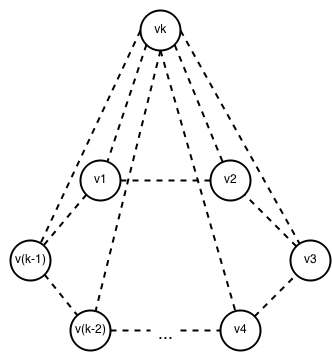
\includegraphics[scale=0.45]{3_1}
\par\end{center}%
\end{minipage}\hfill{}%
\begin{minipage}[t]{0.5\columnwidth}%
\begin{center}
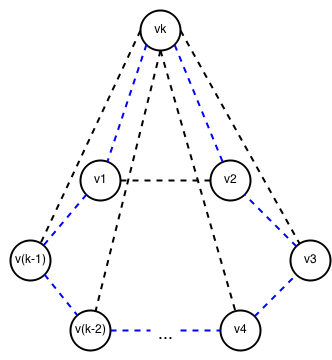
\includegraphics[scale=0.45]{3_2}
\par\end{center}%
\end{minipage}\linebreak{}
\end{figure}

\begin{enumerate}
\item [2.]\setcounter{enumi}{2} Длина цикла $|C| \geqslant k$.
Значит в нем есть не менее $k$ вершин. Так как $G$ $k$-связен,
существует $k$-веер из вершины $v_{k}$ в $k$ вершин цикла $C$,
не обязательно совпадающие с $v_{1},v_{2},\dots,v_{k-1}$, -- обозначим
эти вершины через $x_{1},x_{2},\dots,x_{k}\in C$. Т.е. существует
$k$ попарно непересекающихся простых
путей, ведущих в вершины $x_{1},x_{2},\dots,x_{k}\in C$. Пройдем
по циклу $C$ в одну сторону и разобьем его вершины на $k-1$ непересекающийся блок: $[v_{1},\dots,v_{2}),\ldots, [v_{k-2}, \dots,v_{k-1}), [v_{k-1},v_{1})$ (вершина $v_i$ включена в блок, а вершина $v_{i+1}$ -- нет, она является началом следующего).
Так как блоков -- $k-1$, а путей в веере -- $k$, то по принципу Дирихле, найдется хотя бы один блок, в котором будут заканчиваться два пути веера. Пусть без потери общности $x_{i},x_{j}\in[v_{1},\dots,v_{2})$.
Тогда вместо пути $\left(v_{1},\dots,x_{i},\dots,x_{j},\dots,v_{2}\right)\in C$
возьмем путь $\left(v_{1},\dots,x_{i},\dots,v_{k},\dots,x_{j},\dots,v_{2}\right)$,
включающий два пути веера, а остальную часть цикла $C$ оставим. Получим новый простой цикл $C'$, проходящий через вершины $\left\{ v_{1},v_{2},\dots,v_{k}\right\} $.
\end{enumerate}
\begin{figure}[H]
\begin{minipage}[t]{0.5\columnwidth}%
\begin{center}
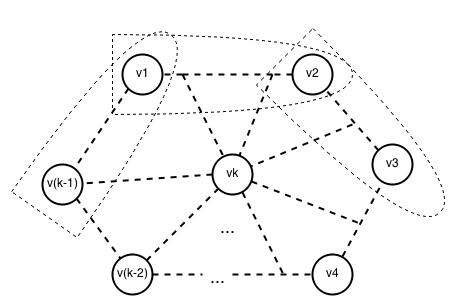
\includegraphics[scale=0.45]{3_3}
\par\end{center}%
\end{minipage}\hfill{}%
\begin{minipage}[t]{0.5\columnwidth}%
\begin{center}
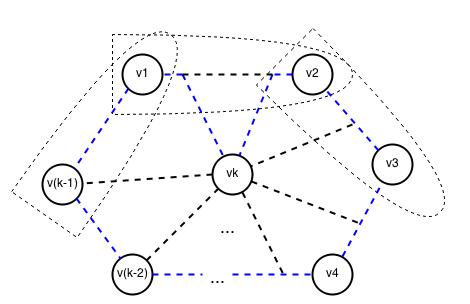
\includegraphics[scale=0.45]{3_4}
\par\end{center}%
\end{minipage}\linebreak{}
\end{figure}

Задача решена.


\end{document}
